\documentclass{article}


% preambulo:
% ! Tex root = mecat-sensorfusion-main

\usepackage[utf8]{inputenc}
% caracteres utf8 (tildes, enie) sin tener que usar comandos



\usepackage[T1]{fontenc}

\usepackage[spanish, es-tabla, es-nodecimaldot]{babel} 
% texto automatico en espaniol
% "tabla" en vez de "cuadro"
% no reemplaza puntos decimales por comas

%% NO AGREGAR PAQUETES ANTES DE ESTO, ES IMPORTANTE QUE BABEL ESTE PRIMERO

%%%%%%%%%%%%%%%%%%%%%%%%%%%%%%%%%
%% PAQUETES EXTRA %%%%%%%%%%%%%%%
%%%%%%%%%%%%%%%%%%%%%%%%%%%%%%%%%

\usepackage{hyperref}					% Hyperlinks on pdf (must be called before Geometry)

\usepackage[a4paper, total={6in, 9in}, footskip=25px]{geometry} 

\usepackage{sansmathfonts}				% Sans Serif equations

\renewcommand*\familydefault{\sfdefault} 	% Sans Serif as default font



\usepackage{subfiles}
\usepackage{xr} % permite referencias a labels de archivos externos con \externaldocument{filename.tex}

\usepackage{amsmath} % PAQUETES DE MATEMATICA
\usepackage{amsfonts}
\usepackage{amssymb}


\usepackage{booktabs} % tablas lindas

\usepackage{units} % permite usar nicefrac
\usepackage{siunitx}
\usepackage{graphicx} % importar imagenes
\usepackage{float} % posicion H para floats
\usepackage[colorinlistoftodos]{todonotes}


\setlength{\parindent}{10pt}			%cuanta sangria al principio de un parrafo
\usepackage{indentfirst}				%pone sangria al primer parrafo de una seccion


% Header style
\usepackage{fancyhdr}
\setlength{\headheight}{15.2pt}
\pagestyle{fancy}
\lhead{31.99 Mecatr\'onica Aplicada}
\chead{TP Sensor Fusion}
\rhead{Roc\'io Parra}
\cfoot{\thepage}


%\usepackage{dblfnote}
%\DFNalwaysdouble 


\hypersetup{
	colorlinks=true,
	linkcolor=blue,
	filecolor=magenta,      
	urlcolor=blue,
	citecolor=blue,    
}

%Para los graficos con multiples imagenes en el mismo float
\usepackage{caption}
\usepackage{subcaption}

\usepackage{wrapfig} % figuras wrappeadas por texto
\usepackage{verbatim} % comment and verbatim environments

\usepackage{listings}
\usepackage{xcolor}

\definecolor{codegreen}{rgb}{0,0.6,0}
\definecolor{codegray}{rgb}{0.5,0.5,0.5}
\definecolor{codepurple}{rgb}{0.58,0,0.82}
\definecolor{backcolour}{rgb}{0.95,0.95,0.92}


\lstdefinestyle{mystyle}{
	backgroundcolor=\color{white},   
	commentstyle=\color{codegreen},
	keywordstyle=\color{magenta},
	numberstyle=\tiny\color{codegray},
	stringstyle=\color{codepurple},
	basicstyle=\ttfamily\footnotesize,
	breakatwhitespace=false,         
	breaklines=true,                 
	captionpos=b,                    
	keepspaces=true,                 
	numbers=left,                    
	numbersep=5pt,                  
	showspaces=false,                
	showstringspaces=false,
	showtabs=false,                  
	tabsize=2
}

\lstset{style=mystyle}

 



\begin{document}

%\newgeometry{total={6in, 8in}, footskip=50px} % margenes default para la caratula
% caratula:
% !Tex root = mecat-sensorfusion-main

\begin{titlepage}
\newcommand{\HRule}{\rule{\linewidth}{0.5mm}}
\center
\mbox{\textsc{\LARGE \bfseries {Instituto Tecnol\'ogico de Buenos Aires}}}\\[1.5cm]
\textsc{\Large 31.99 Mecatr\'onica Aplicada}\\[0.5cm]


\HRule \\[0.6cm]
{ \Huge \bfseries Trabajo Pr\'actico:  

 Sensor Fusion
%
%Realimentados\vspace{0.2cm} 
 }\\[0.4cm] % Title of your document
\HRule \\[1.5cm]

\vfill
{\large

%\emph{Grupo 2}\\
%\vspace{3px}

\begin{tabular}{lr} 	
\textsc{Parra}, Roc\'io  & 57669 \\
\end{tabular}

\vspace{50px}

\emph{Profesores}\\
\vspace{3px}
\textsc{Perfumo}, Lucas Alberto\\ 
\textsc{Fortunatti}, Nelson Ariel\\
\vspace{100px}

\begin{tabular}{ll}

Presentado: & 23/10/2020\\


\end{tabular}

}

\vfill

\end{titlepage}

%\newgeometry{a4paper, total={7in, 9.25in}, footskip=25px}
% indice:
\tableofcontents
%\newpage

\section{Consigna}
\begin{itemize}
	\item Diagrama de bloques de los dos programas
	\item Sincronizaci\'on
	\item Presentar gr\'aficos obtenidos
	\item Video
\end{itemize}

\section{Funcionamiento}

\subsection{Programa del microcontrolador}

\begin{figure}[ht]
	\centering
	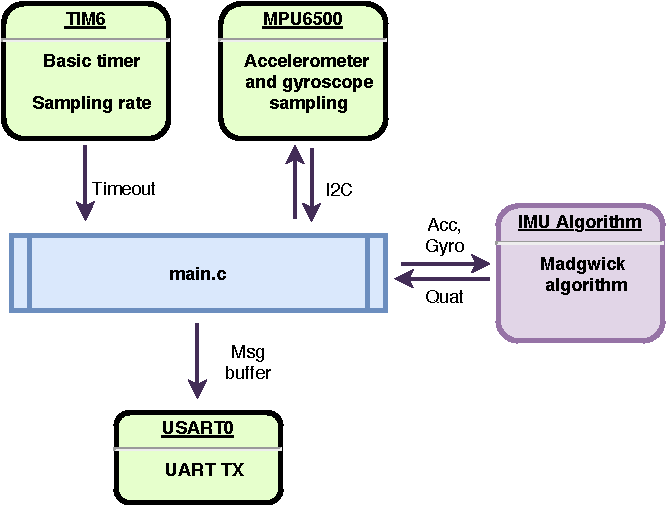
\includegraphics[width=0.7\textwidth]{imgs/cprog.pdf}
	\caption{Diagrama de bloques del programa del microcontrolador}
	\label{fig:cprog}
\end{figure}

\subsection{Programa de la computadora}

\begin{figure}[ht]
	\centering
	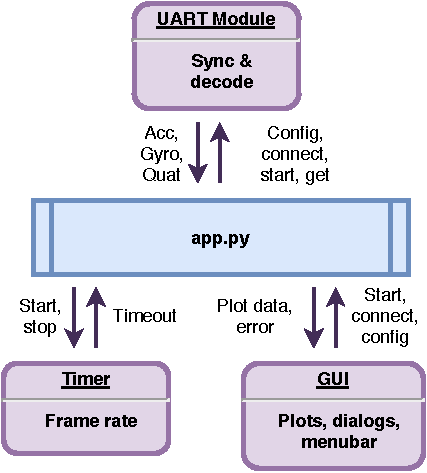
\includegraphics[width=0.5\textwidth]{imgs/pyprog.pdf}
	\caption{Diagrama de bloques del programa de la computadora}
	\label{fig:pyprog}
\end{figure}



\section{Sincronizaci\'on}

El env\'io de datos desde el microprocesador a la computadora se realiz\'o v\'ia UART, con un baudrate de 115200, sin paridad, 8 bits por palabra y un stopbit. No se implement\'o ning\'un mecanismo de acknowledgement por parte del programa en la computadora, ya que los datos son enviados en tiempo real, y reenviar paquetes comprometer\'ia esta caracter\'istica.

La sincronizaci\'on se realiz\'o estructurando los mensajes de la siguiente manera:
\begin{itemize}
	\item 1 byte con la letra `A' (por aceletr\'ometro) en ASCII
	\item 3 floats de 32 bits, indicando las componentes $x$, $y$ y $z$ del aceler\'ometro, en ese orden
	\item 1 byte con la letra `G' (por giroscopio) en ASCII
	\item 3 floats de 32 bits, indicando las componentes $x$, $y$ y $z$ del giroscopio, en ese orden
	\item 1 byte con la letra `Q' (por cuaterni\'on en ingl\'es, \textit{quaternion}) en ASCII
	\item 4 floats de 32 bits, indicando las 4 componentes de la aproximaci\'on del cuaterni\'on representando la posici\'on de MPU
\end{itemize}

De esta manera, cada mensaje cuenta con 40 bytes de datos (3+3+4=10 floats, cada uno de cuatro bytes) y 3 bytes de sincronizaci\'on. El programa en la computadora detecta la presencia de un mensaje v\'alido a partir de estos tres caracteres en la posici\'on  adecuada. Esta tarea se realiza en un \emph{thread} independiente, que constantemente busca nuevos mensajes y los guarda en una \emph{queue}, hasta ser detenido por un evento de \emph{stop}, o detectar un error en el puerto serie.

A continuaci\'on se muestra la totalidad del c\'odigo correspondiente a este \emph{thread}. 

\begin{center}
	\begin{lstlisting}[language=Python]
		def uart_sync(self):
			try:
				# ignore all old msgs
				self.ser.flush()
				
				# wait for the next whole msg
				buff = self.ser.read(MSG_SIZE)
				
				# run until told to stop
				while not self.end.is_set():
					
					# check whether the msg fits the format
					agq = buff[0::FLOAT_SIZE * 3 + 1][:3]
					try:
						agq = agq.decode(encoding='ascii')
					except UnicodeDecodeError:
						pass
					
					# if the msg fits the format, queue it
					if agq == 'AGQ':
						self.q.put(buff)
						buff = self.ser.read(MSG_SIZE)
					
					# else drop first byte and read one more
					else:
						buff = buff[1:] + self.ser.read(1)
			
			except (serial.SerialException, serial.SerialTimeoutException) as e:
				# if there was a problem with the serial port, report it
				self.q.put(e) 
			else:
				# if no exceptions were raised, discard all previous msgs
				self.q = Queue(maxsize=QUEUE_SIZE)
			finally:
				# mark event as read
				self.end.clear()
	\end{lstlisting}
\end{center}



\end{document}
